\documentclass[../main.tex]{subfiles}

\graphicspath{{\subfix{../images/}}}
\begin{document}
\chapter{GraphQL Application Architecture: An Overview}
\section{Various GraphQL architecture approaches}
\subsection{GraphQL application architecture}
GraphQL is just a specification that set out how a GraphQL server should behave.
This essentially means, a set of guidelines will be defined by any GraphQL based application - on how requests and responses to be handled by the server.


The guidelines generally include:
\begin{itemize}
  \item What are the supported protocols?
  \item Which format of data can be acceptable for the server?
  \item Which format of response is possible for the server to return? etc.
\end{itemize}

\subsubsection{The GraphQL mindset}
The request from a GraphQL client to the GraphQL server is known as Query.
GraphQL is transport-layer agnostic. That is, GraphQL actually is agnostic with respect to how data flows over the network. GraphQL server can work with protocols other than HTTP as well. To quote a few, WebSockets and TCP. But, the most widely used one is HTTP indeed.
GraphQL is neutral to databases. That is, we are free to use GraphQL with SQL or NoSQL databases or even the combination of both!

\subsubsection{Various GraphQL app architecture possibilities}
A GraphQL server can be created using either of the methods being listed below –

\begin{enumerate}
\item GraphQL server with a connected database
\item GraphQL server that integrates existing (possibly legacy) systems
\item Hybrid approach – which is a mix of the above two approaches
\end{enumerate}

\subsection{GraphQL Server with Connected Database}
In this architecture, we can find GraphQL Servers with a tightly coupled/integrated database.
Upon receiving a query from the client, the GraphQL server will first make sure reading the request payload and then fetching the required data from the database.
This is known as resolving the query which in turn results in a response from the GraphQL server.
The response is returned to the client and it adheres to the format being specified in the GraphQL specification that is provided by the Schema and the Type system.
This kind of architecture can often be used in projects that start from scratch.

\begin{figure}[h!]
\centerline{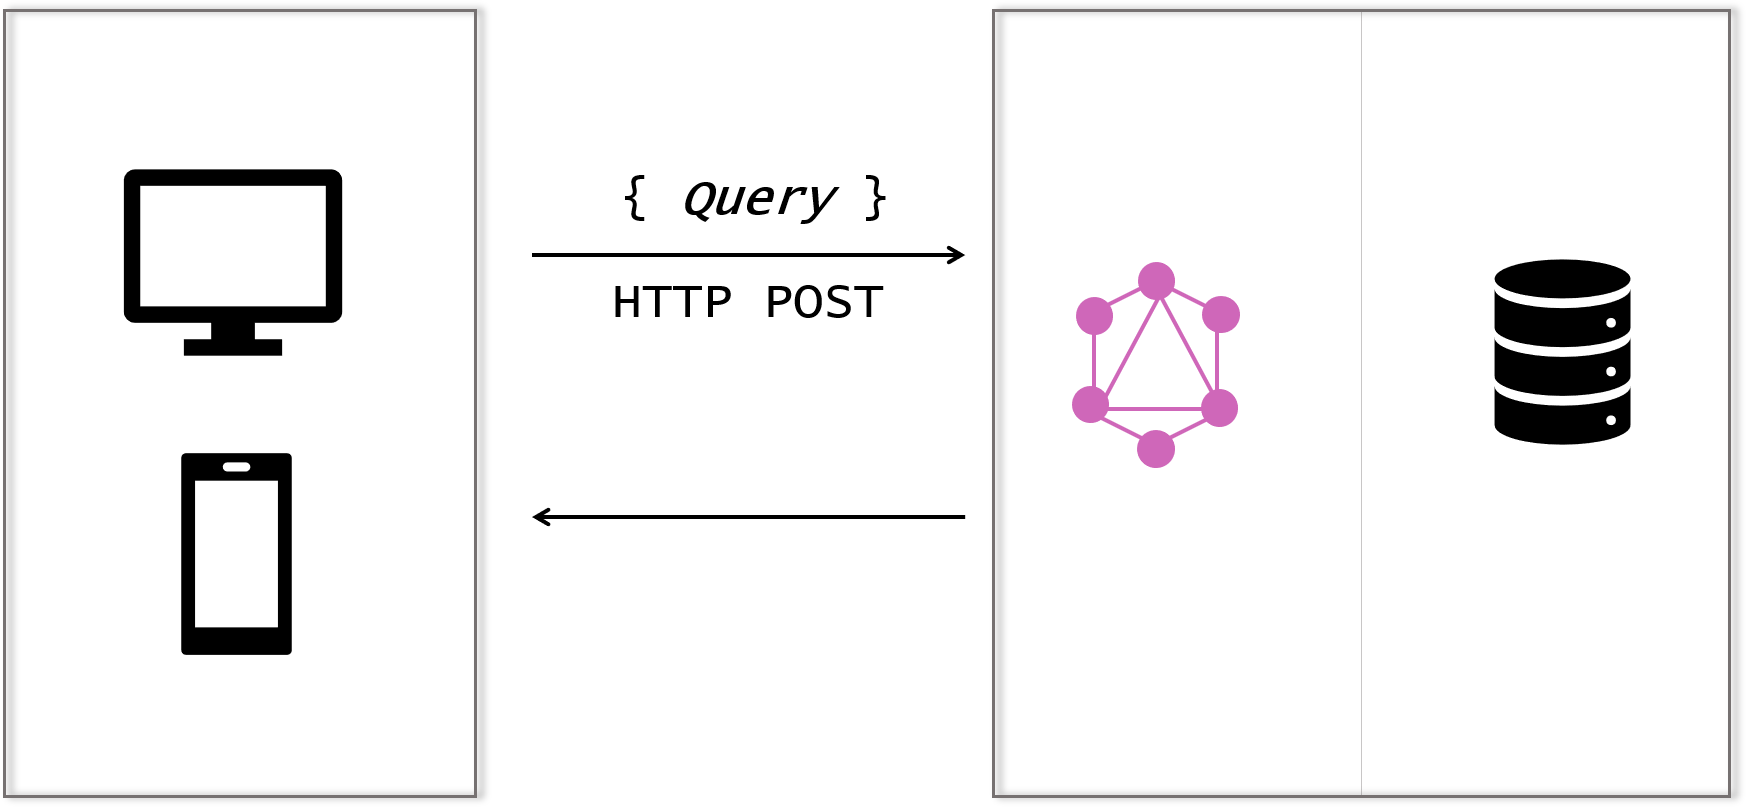
\includegraphics[width=150mm]{GQLArchi11601287761696.png}}
\caption{GraphQL Server with a Connected DataBase}
\label{fig:GraphQL-Server-with-a-Connected-DataBase}
\end{figure}

In the diagram being shown above, the GraphQL server and the database (SQL or NoSQL) are made to be available on a single node. The Client (desktop or mobile) communicates with the GraphQL server over HTTP. The server processes the request fetches/retrieve data from the DB and, returns it finally to the client.

\subsection{GraphQL server integrating the existing Systems}
This approach would be much helpful for the companies that have legacy infrastructure and possess a collection of different APIs. GraphQL can be employed in this kind of architecture to unify microservices, legacy infrastructure, and even third-party APIs.
Observe the below block diagram:

\begin{figure}[h!]
\centerline{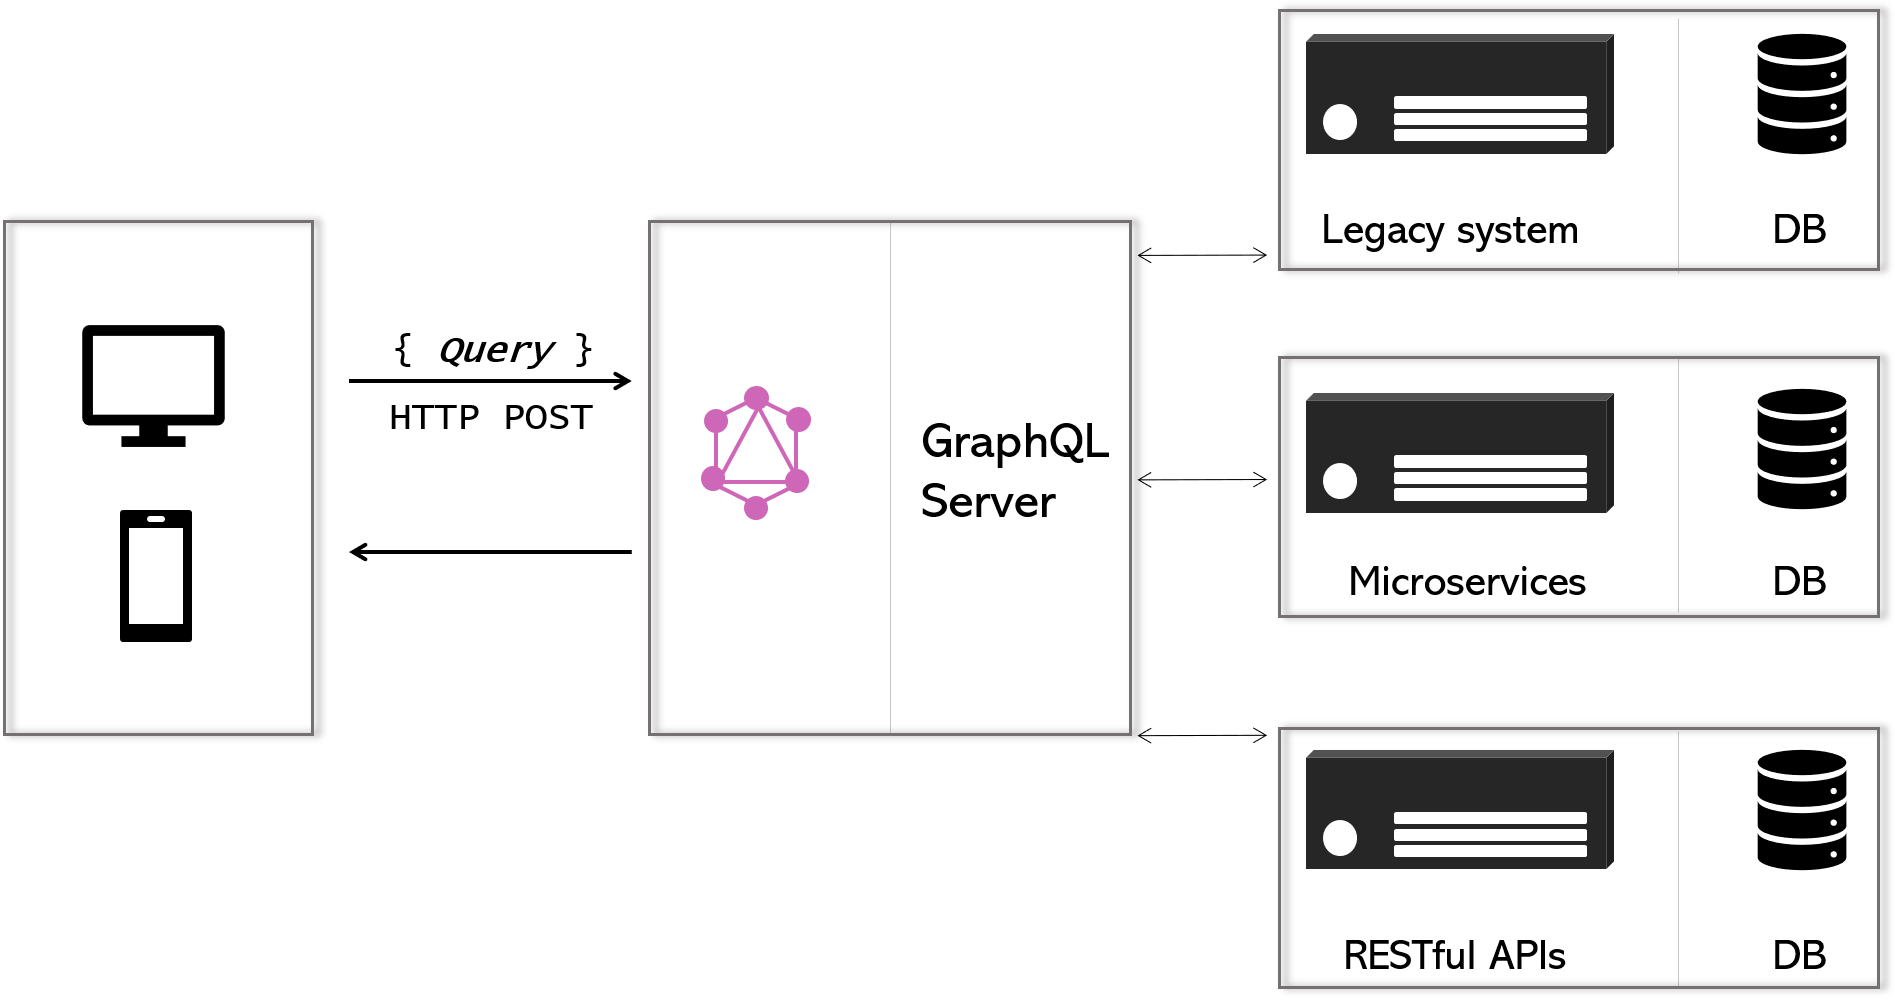
\includegraphics[width=150mm]{GQLArchi21601287889595.png}}
\caption{GraphQL server integrating the existing Systems}
\label{fig:GraphQL-server-integrating-the-existing-Systems}
\end{figure}

In the given diagram, GraphQL Server acts as an interface between the client and the existing systems. Client applications reach out to the GraphQL server which in turn, resolves the query and gets data from the existing APIs, and renders the response back to the client applications.

\subsection{Hybrid Approach}
Finally, we can put the first two approaches together that is, the dedicated DB approach and the integrated legacy systems approach, to build a GraphQL server. In this architecture, the GraphQL server shall resolve the requests being received. It will then, retrieve data either from the connected database or from the integrated APIs.

\begin{figure}[h!]
\centerline{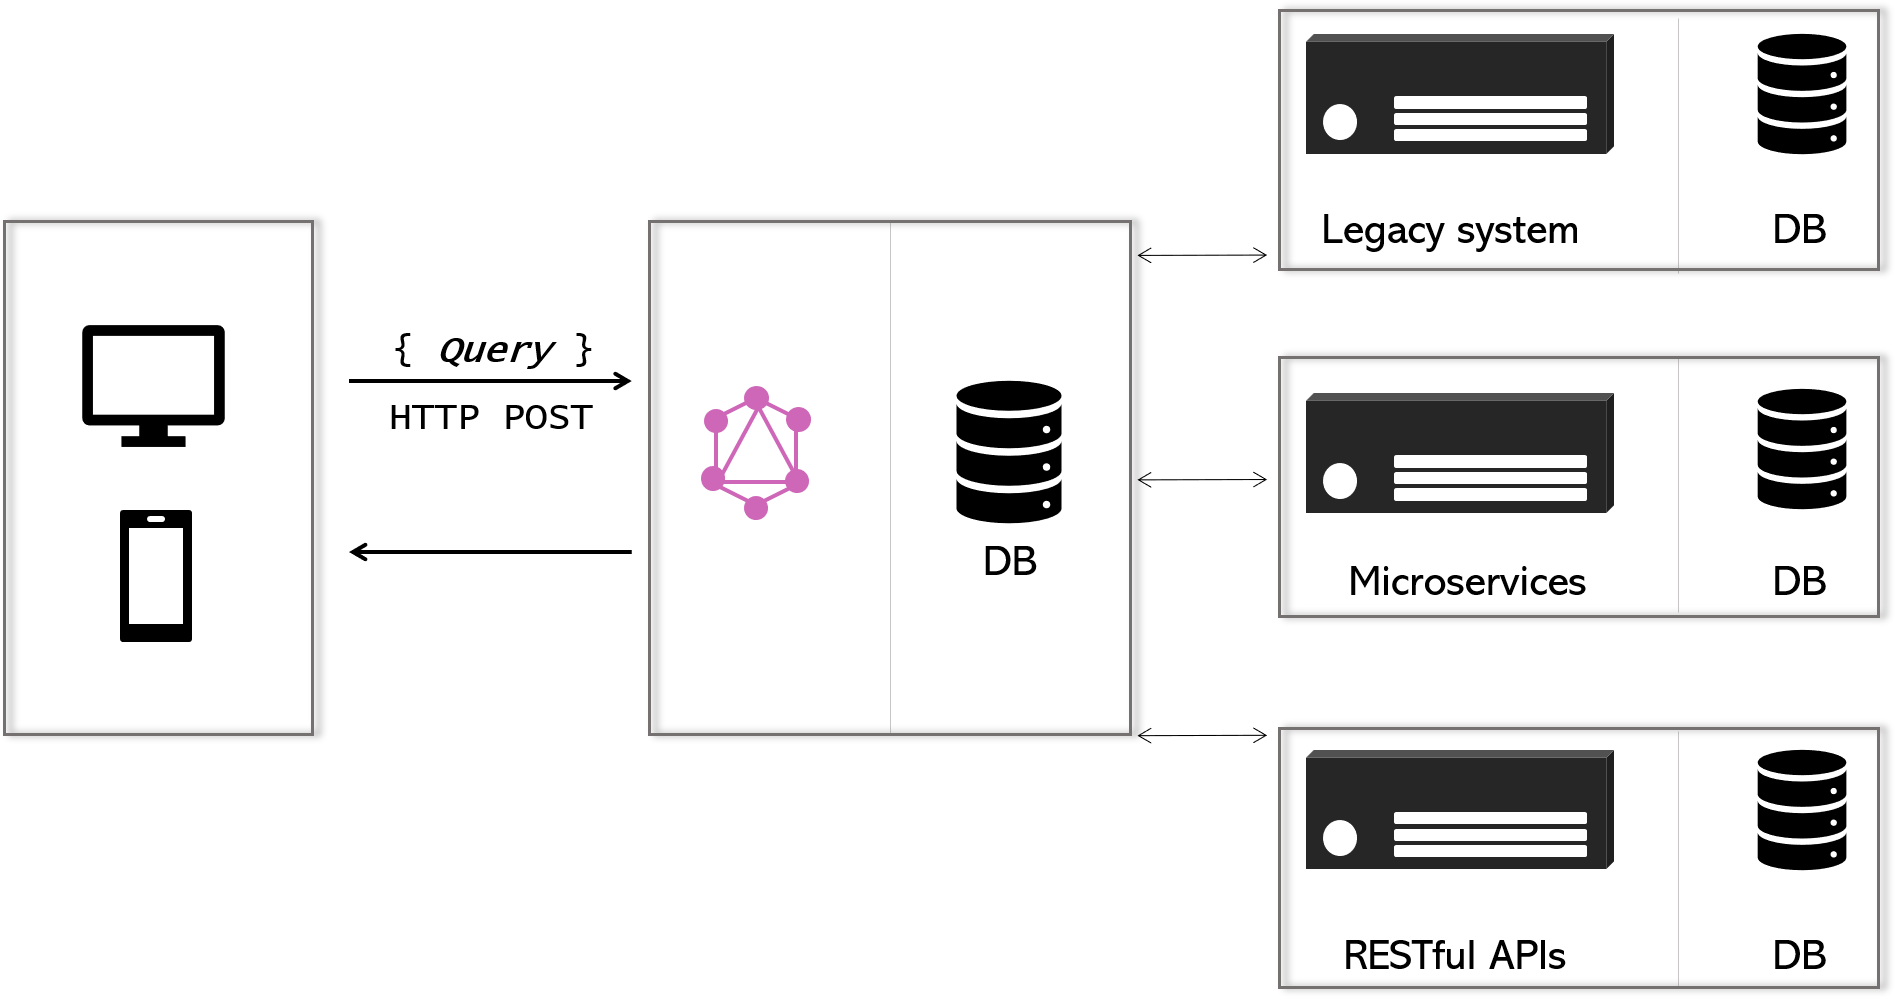
\includegraphics[width=150mm]{GQLArchi31601287943645.png}}
\caption{Hybrid Approach}
\label{fig:Hybrid-Approach}
\end{figure}

\section{GraphQL Application Components}
Just like any other full-stack application, a GraphQL based application will also have the following types of components:
\begin{itemize}
  \item Server-side components
  \item Client-side components
\end{itemize}
\subsection{GraphQL Application Components - Server Side}
Any GraphQL server will contain the following components.

\begin{enumerate}
  \item { \textbf{Schema}: GraphQL schema is the heart of any GraphQL server. The schema is a description file that contains the types that are available with the system and the various set of operations that can be performed on those types. In other words, GraphQL helps to expose the various “data resources” that are available to the clients connected to the GraphQL server.}
  \item { \textbf{Query}: GraphQL query is nothing but the request being initiated by the GraphQL client to the GraphQL server. The response to the request can be from various data sources like databases or other legacy REST APIs. An important point to be noted here is, GraphQL query is \textbf{declarative} (easy for us to predict the content that will be received by the client on seeing the query itself) by nature and helps to query the GraphQL server in a precise manner.}
  \item { \textbf{Resolver}: Resolvers are nothing but the entities which provide instructions that are required to turn a GraphQL query/operation into data. They actually “resolve” the query and return data by defining various resolver functions that correspond to the schema.}
\end{enumerate}

These server-side components help the GraphQL server to parse the queries that are coming from the GraphQL client applications and to generate the relevant response. 
We are aware that GraphQL is a specification and has got multiple implementations. We have a variety of languages supporting the creation of the GraphQL server. In this course, we shall see the Spring Boot way of creating a GraphQL server.

\subsection{GraphQL Application Components - Client Side}
Like server-side components, there are various components on the client-side as well. Take a look at the below client-side components.

\begin{enumerate}

  \item {\textbf{GraphQL Playground}: A browser-based interface that helps to edit and testing GraphQL queries/mutations/subscriptions. }
  \item {\textbf{Apollo Client}: Tool/library that helps to build GraphQL client applications and can integrate well with any JavaScript-based front-end. }
  \item {\textbf{Postman}: Tool to test REST API endpoints. The recent versions of Postman have support for sending GraphQL queries as well. }

\end{enumerate}

We have got an idea of GraphQL's client and server-side components. Before getting deeper, let's have a look at how happens the interaction between a GraphQL client and the GraphQL server (Spring Boot based).

\begin{itemize}
\item {The web server can be built on Spring Boot.}
\item {A request is made to the Spring Boot GraphQL Server by a GraphQL client. The client application can either be a ReactJS application (the one that is built with the help of Apollo Client library) or GraphQL playground or even GraphiQL browser application.}
\item {The query will get parsed and validated against the schema that is defined in the server.}
\item {If the request passes the validation, the associated resolver methods will be executed.}
\item {The resolver-contained code then will fetch data from a database or an API.}
\item {Finally, the result gets rendered back to the client that initiated the request.}
\end{itemize}

\printglossaries
\end{document}
